\chapter{Justificaci'on}
\section{¿Porqu'e una aplicaci'on m'ovil?}
\subsection{Las TIC en la educaci'on}
De acuerdo con Teemu Leinonen (2005) en la educaci'on el uso de las nuevas tecnolog'ias de la informaci'on ha pasado por las siguientes etapas:

\begin{figure}
	\begin{center}
		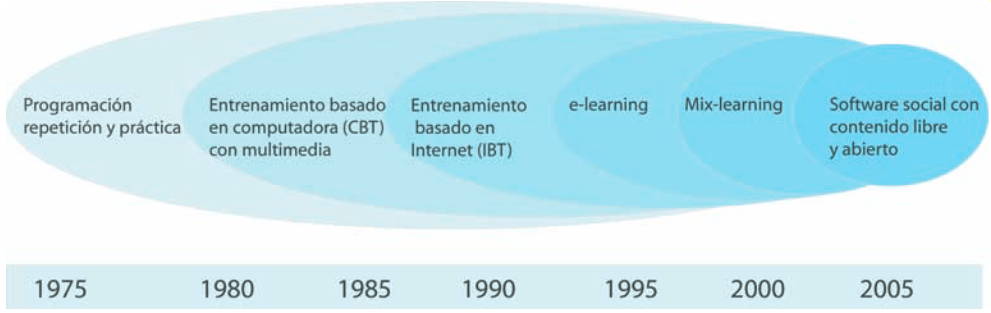
\includegraphics[scale=0.5]{img1.png} 
		\caption{Evoluci'on de las TIC en la educaci'on. (Basado en Leinonen 2005)}
		\label{tic}
	\end{center}
\end{figure}

Esta evoluci'on muestra como cada vez el aprendizaje va utilizando m'as tecnolog'ia; pasando de ser 'esta simplemente una herramienta de apoyo, hasta ser la plataforma a trav'es de la cual se presentan los contenidos y eval'uan los conocimientos. 

Mix-Learning. La etapa posterior al e-learning es la aplicaci'on de una mezcla de sus herramientas con sistemas educativos tradicionales. La finalidad es dirigir m'as espec'ificamente los contenidos a los estudiantes. Es as'i que el Blend Learning, Mix Learning o Hybrid Learning se presenta como ``la combinaci'on efectiva de los diferentes modelos de reparto, modelos de ense'nanza y modelos de aprendizaje" (Heinze, A.y C. Procter, 2004, p 1.).

\subsection{M-Learning en la educaci'on}
Seg'un la Organizaci'on de las Naciones Unidas para la Educaci'on la Ciencia y la Cultura (UNESCO, 2012) existen 5.9 billones de suscripciones de tel'efonos m'oviles en el mundo, contra los 7.04 billones de habitantes. Adem'as, en el a'no 2020 los dispositivos m'oviles ser'an la principal herramienta de conexi'on a internet para la mayor'ia de la poblaci'on; en Jap'on, actualmente el 75\% de su poblaci'on tiene un dispositivo m'ovil como primer medio de acceso a internet, (SCOPEO, 2011). 

Asimismo, en a'nos recientes el uso de la tecnolog'ia m'ovil para fines educativos, conocido como m-learning, ha tenido un gr'an desarrollo en la educaci'on superior, ya que existen universidades de Europa y Am'erica que cuentan con sistemas de educaci'on m'ovil, (Traxler, 2007).

\subsection{La importancia de la programaci'on orientada a objetos}
La programaci'on Orientada a Objetos surge como el paradigma que permite manejar ampliamente las nuevas plataformas que garanticen desarrollar aplicaciones robustas, portables y reutilizables que puedan ofrecer una soluci'on a largo plazo en un mundo donde los cambios se dan a cada momento.

El desarrollo de programas orientados a objetos es un enfoque diferente del mundo inform'atico. Implica la creaci'on de modelos del mundo real y la construcci'on de programas inform'aticos basados en esos modelos.

La importancia de esta programaci'on radica en que, favorece la creaci'on de programas de calidad, fuerza en mantenimiento, en extensi'on y reutilizaci'on de programas. Est'a basada en el modo de pensar del hombre y en el modo de trabajar de la m'aquina.

Es muy importante que los estudiantes sean capaces, no s'olo de manejar los conceptos de orientaci'on a objetos, sino tambi'en de aplicarlos de manera efectiva en el desarrollo de programas.

\section{¿D'onde se aplicar'a?}
